 \section{Mappings} \label{sec:mappings}
As previously discussed, objects simulated in \sofa, like the liver in Figure \ref{fig:liver-multimodel}, typically rely on several models: one for the internal model, one for collision, and one for the visual rendering. 
To enforce consistency, one of them, typically the internal model, acting as the master, imposes its displacements to slaves (typically the visual model and the collision model), using \textit{mappings}.
Mapped model can be masters of other models in turn, creating a hierarchy whith the independent DOFs at the root.
Figure \ref{fig:hierarchy} illustrates the hierarchies of two objects. The visual models, in additional branches, are omitted for clarity. When contact models collide, additional geometry is necessary to model the contacting points.
This additional geometry is represented in an additional level connected to the models, as depicted in the figure. 


The positions $\vec x_c$ of a child model are computed by the mapping based on the positions $\vec x_p$ of the master using a function $\JNL$. 
\begin{equation} %\label{eq:mapV}
\vec x_c =\JNL(\vec x_p)
\end{equation}
% In the particular case of a FEM model, this mapping function can rely on the underlying interpolation of the model. 
% 
% 
% These mapping are implemented in a very generic way and allows the control of any kind of slave model $\vec x_1 = \JNL_1(\vec x_0)$ given the position of a master model $\vec x_0$ . 
The velocities can be mapped in a similar way:
\begin{equation}
\vec v_c = \mat J \vec v_p
\end{equation}
The Jacobian matrix $\mat J = \frac{\partial \vec x_c}{\partial \vec x_p}$ encodes the linear relation between the parent and child velocities.
It also holds on accelerations, with an additional offset due to velocities when the position mapping $\JNL$ is nonlinear.
In linear mappings, operators $\JNL$ and $\J$ are the same, otherwise $\JNL$ is nonlinear with respect to $x_p$ and it can not be written as a matrix.
For surfaces embedded in deformable cells, matrix $\J$~contains the barycentric coordinates (it corresponds to linear interpolation in FEM).
For surfaces attached to rigid bodies, each row of the matrix encodes the usual relation $v = \dot o + \omega \times (x-o)$ for each vertex. 

The positions and the velocities are propagated top-down in the hierarchy. 
Conversely, the forces are propagated bottom-up, up to the independent DOFs, where Newton's law $\vec f=\M\vec a$ is applied. 
Given forces $\vec f_c$ applied to a child model, the mapping computes and accumulates the equivalent forces $\vec f_p$ applied to its parent. 
Since equivalent forces must have the same power, the following relation holds:
$$
\vec v_{p}^T \vec f_p = \vec v_c^T \vec f_c
$$
The kinematic relation $\vec v_{c} = \J \vec v_{p}$ allows us to rewrite the previous equation as
$$
\vec v_{p}^T \vec f_{p} = \vec v_{p}^T \J^T \vec f_c
$$
Since this relation holds for all velocities $\vec v_p$, the principle of virtual work allows us to simplify the previous equation to obtain:
\begin{equation} \label{eq:mapF}
\vec f_{p} = \J^T \vec f_c
\end{equation}
When a model has several children, each child accumulates its contribution to the parent forces using its mapping. 
This hierarchical kinematic model allows us to compute displacements and to apply forces at all levels.
%
\begin{figure}
 \centering
 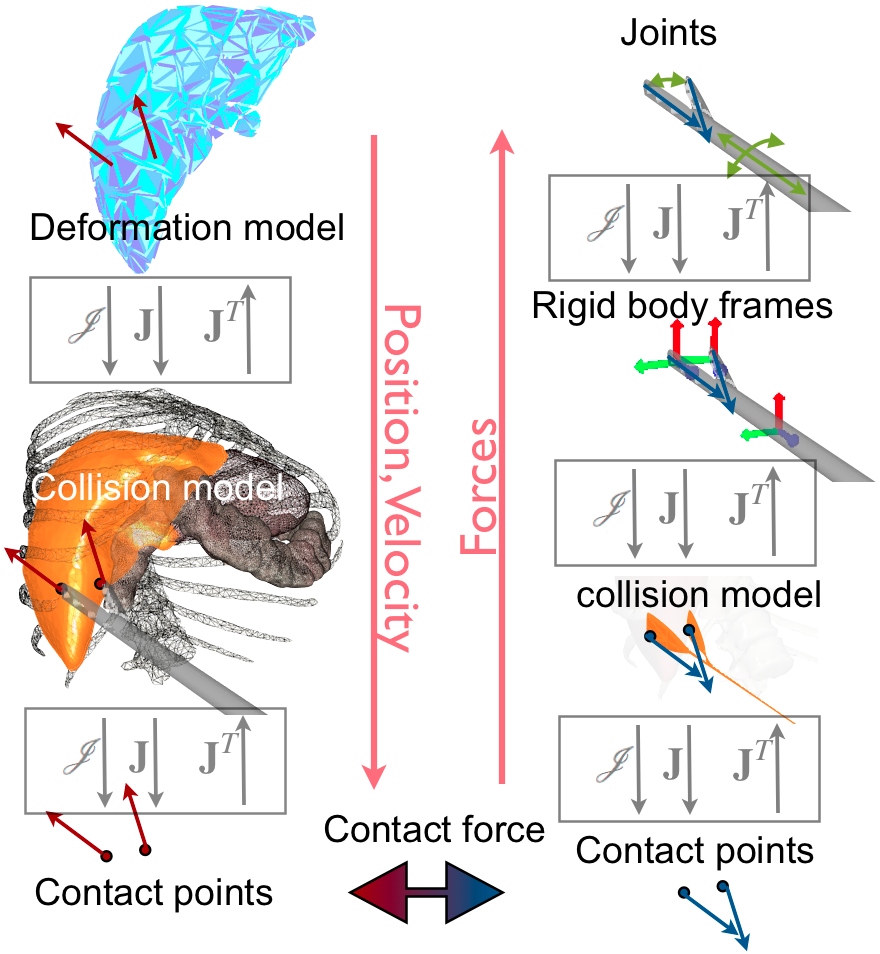
\includegraphics[width=0.9\linewidth]{MappingScheme.png}
 \caption{Mappings from the DOFs to the contact point. Right (top to bottom): The Mechanical model of the liver is based on Finite Element model. A triangular mesh is mapped for collision detection with the surface. The two contact points found by the collision detection (with the grasper) are mapped on the collision model. 
 Left (bottom to top): the contact points are also mapped on the collision model of the grasper. This collision model is a simplification of the grasper shape and is mapped on the rigid body frames. The motion of these frame is mapped on the state of the joints which are the independent DOFs of the grasper.
}
 \label{fig:hierarchy}
\end{figure}
%
So far, $22$ variants of mappings have been implemented to attach models to rigid objects and deformable primitives such as tetrahedra, hexahedral grids, splines, blended frames, flexible beams and scalar fields.
Mappings are also be used to connect generalized coordinates, such as joint angles, to world-space geometry, as in the grasper of Figure~\ref{fig:hierarchy}.


%% attacher de la g�om�trie
%
%
%They are not independent variables, since the positions and velocities are bound to the independent DOF.
%We say that a child geometrical model $1$ is \textit{mapped} from its parent model $0$,
% using a kinematic operator which we call \textit{mapping}. It implements the kinematic relations:
%\begin{eqnarray*} %\label{eq:mapV}
%\vec x_1 &=&\JNL_1(\vec x_0)\\ 
%\vec v_1 &=& \mat J_1 \vec v_0
%\end{eqnarray*}
%Mappings allow to attach polygonal shapes (like the tool shape in Figure~\ref{fig:hierarchy}, with point DOFs) to rigid bodies (with frame DOFs) using local coordinates, or to embed the shapes in deformable cells using barycentric coordinates (like the deformable liver in Figure~\ref{fig:hierarchy}), among other possibilities.
%Matrix $\mat J_1 = \frac{\partial \vec x_1}{\partial \vec x_0}$ encodes the linear relation between the parent and child velocities.
%It also holds on accelerations, with an additional offset due to velocities when the position mapping \JNL is nonlinear.
%In linear mappings, operators \JNL and \J are the same, otherwise \JNL is nonlinear with respect to $x_0$ and it can not be written as a matrix.
%For surfaces embedded in deformable cells, matrix \J~contains the barycentric coordinates. 
%For surfaces attached to rigid bodies, each row of the matrix encodes the usual relation $v = \dot o + \omega \times (x-o)$ for each vertex. 
%% Similarly, skins around articulated bodies involve, at each vertex, the weighted  contributions of the rigid bodies. 


%% g�om�trie suppl�mentaire d�e aux contacts
%When shapes collide, additional geometry is necessary to model the contact.
%For instance, when an edge intersects or closely approaches another one, a contact force is typically applied to the intersection point or to the pair of points.
%The points are defined using their barycentric coordinates with respect to the edge vertices. 
%% Other relations can be used, depending on the kind of geometrical primitives in contact.
%This additional geometry can be represented in another geometrical layer connected to the shape by a mapping, as illustrated in the bottom of Figure~\ref{fig:hierarchy}.
%% This layer is also connected to the shape using mappings:
%% \begin{eqnarray*} %\label{eq:mapV}
%% x_2 &=&\JNL_2(x_1)\\ 
%% v_2 &=&J_2 v_1 
%% \end{eqnarray*}
%
%We generalize this approach to tree-like hierarchies of geometries, with the independent DOFs at the root. 
%For instance, the independent DOFs may have two children, one for collision using a coarse mesh, and the other for rendering using a finer mesh.
%The hierarchy have more levels, for instance, to attach collision spheres to a mesh embedded in a deformable grid. 
%The synchronization between these models is automatically guaranteed by their attachment to their common ancestor, using graph visitors as explained in Section~\ref{sec:visitors}.
%Positions and velocities are propagated top-down in the hierarchy. Conversely, the forces are propagated bottom-up, up to the independent DOFs, where Newton's law $f=ma$ is applied. 
%Given forces $f_c$ applied to a child model, the mapping computes and accumulates the equivalent forces $\vec f_p$ applied to its parent. 
%Since equivalent forces must have the same power, the following relation holds:


% In implicit simulation methods, one needs to consider force changes $\vec{df}$ corresponding to small displacements $\vec{dx}$ of the independent DOF.
% This involves the forces applied to the independent DOF, but also the forces are applied to mapped DOFs.
% Let $0$ denote the independent DOF.%, and $n$ a level mapped through $n$ mappings indexed from $0,1$ to $n-1,n$.
% At each hierarchy node $i$, let $\mat K_{ii}$ be the stiffness matrix corresponding to the forces applied to the local DOF.
% The local displacement is :
% \begin{equation} \label{eq:displacementsTopDown}
%  \vec{dx}_{i} = \prod_{j=1}^{i}\mat J_{j,j-1} \vec{dx}_{0}
% \end{equation}
% where $\prod_{j=1}^{i}\mat J_{j,j-1} = \mat J_{i,i-1}...\mat J_{1,0}$ is the product of the matrices of the mappings in the path from the independent DOF to node $i$.
% The matrix-vector product can be efficiently computed during one top-down traversal of the hierarchy, with one matrix-vector product at each level, without any matrix-matrix product.
% Conversely, the resulting force change on the independent DOFs is:
% \begin{equation} \label{eq:forcesBottomUp}
%  \vec{df}_{0} = \left( \prod_{j=1}^{i}\mat J_{j,j-1} \right)^T \vec{df}_{i}
% \end{equation}
% where $\left( \prod_{j=1}^{i}\mat J_{j,j-1} \right)^T = \mat J_{1,0}^T...\mat J_{i,i-1}^T$ is the product of the transposed matrices of the mappings in the path from node $i$ to the independent DOF.
% This matrix-vector product can be efficiently computed using matrix-vector products during one bottom-up traversal of the hierarchy.

%Figure~\ref{fig:liver-mechanical-spheres} shows a sphere-based collision model attached to the mechanical model of Figure~\ref{fig:liver-mechanical}. 
%The position vector of the collision model is the set of 3d coordinates of the sphere centers, defined by their barycentric coordinates stored in the BarycentricMapping.
%\begin{figure}
% \centering
% 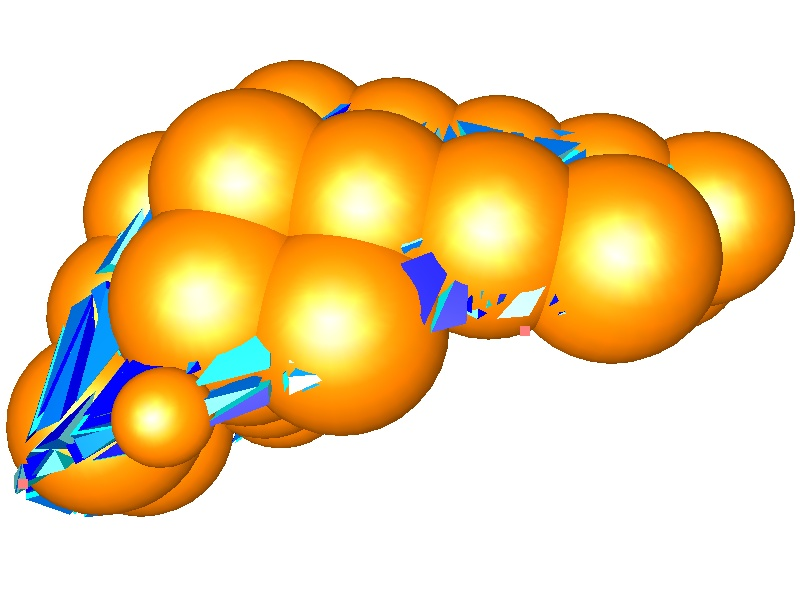
\includegraphics[width=0.4\linewidth]{liver-spheres-superimposed.jpg}
% 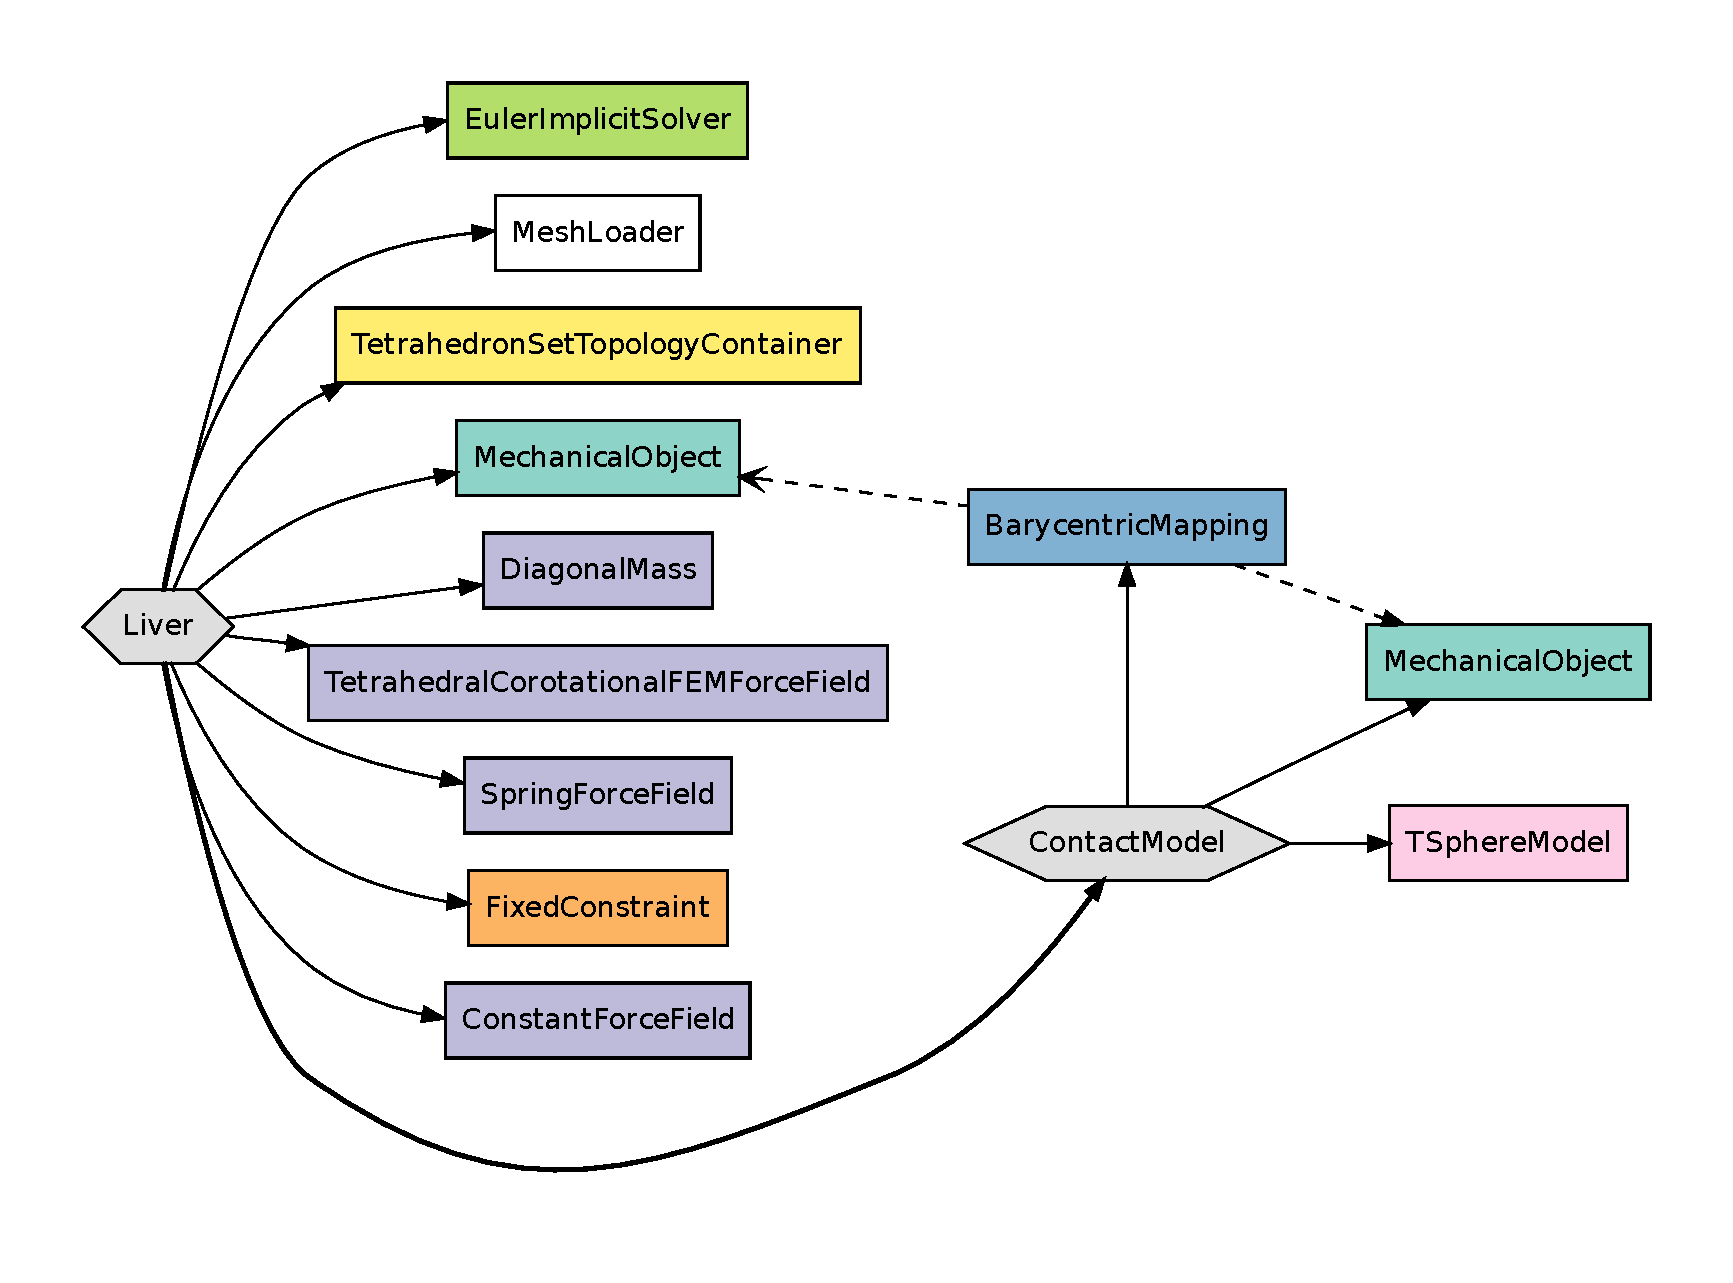
\includegraphics[width=0.56\linewidth]{liver-spheres.pdf}   % generated from ps using: dvipdf -dEPSCrop
% \caption{Left: mechanical (in blue) and collision (in yellow) models of a liver. Right: the corresponding scene graph. The plain arrows denote hierarchy, while the stippled arrows represent connections.}
% \label{fig:liver-mechanical-spheres}
%\end{figure}




